% -*- coding: UTF-8 -*-
% hurlex-chapt10.tex
% hurlex 开发文档 第10章内容

\section {虚拟内存管理的实现}

\par 这章将详细研讨虚拟内存管理的实现。

\par 上一章谈到,虚拟的页面每页占据4KB,按页为单位进行管理。物理内存也被分页管理,按照4KB分为一个个物理页框。虚拟地址到\allowbreak
物理地址通过由页目录和页表组成的二级页表映射,页目录的地址放置在CR3寄存器里。

\par 至此,我们彻底揭开了x86下32位寻址的面纱,下图描述了地址转换的完整过程。

\begin{figure}[ht]
      \centering
      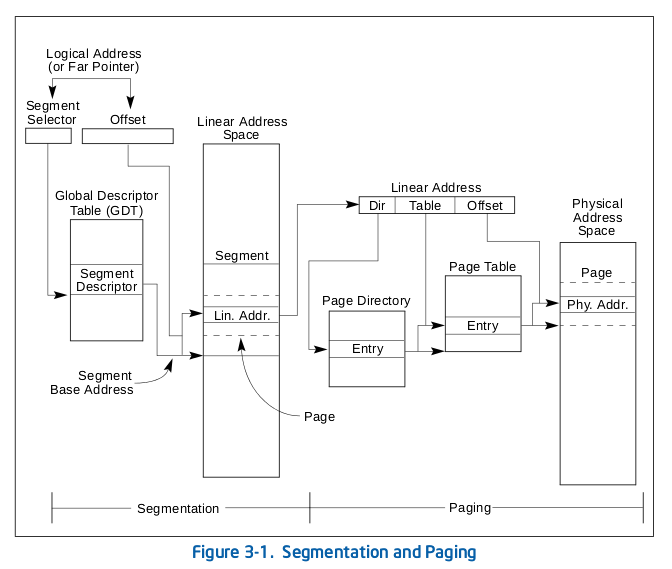
\includegraphics[scale=0.6]{picture/chapt10/ADDR_TRAN.png}
      \caption{段页式转换}
\end{figure}

\par 因为我们使用了Intel平坦模式的内存模型,所以之前的分段机制是被"绕过去"的,所以分页的管理就成了内存管理的核心了。首先是\allowbreak
内核自身地址的映射,Linux采用的是方案是把内核映射到线性地址空间3G以上,而应用程序占据线性地址空间0-3G的位置。我们的内核采取\allowbreak
和Linux内核一样的映射,把物理地址0从虚拟地址0xC0000000(3G)处开始往上映射,因为我们只管理最多512MB的内存,所以3G-4G之间\allowbreak
能完全的映射全部的物理地址。采取这个映射后,物理地址和内核虚拟地址满足以下关系:

\par 物理地址 + 0xC0000000 = 内核虚拟地址

\par 但是采用这个设计的话会给已有的代码带来什么麻烦呢?

\par 我们先引入VMA(Virtual Memory Address)和LMA(Load Memory Address)这两个概念。其中VMA是链接器生成可执行文件时的偏移\allowbreak
计算地址,而LMA是区段所载入内存的实际地址。通常情况下的VMA是等于LMA的。使用以下命令可以查看内核文件的区段信息:
\begin{Verbatim}[frame=single]
    objdump -h hx_kernel
\end{Verbatim}

\par 输出大概是这个样子:

\begin{Verbatim}[frame=single]
hx_kernel:     file format elf32-i386

section:
Idx Name          Size      VMA       LMA       File off  Algn
  0 .text         00003000  00100000  00100000  00000080  2**4
                  CONTENTS, ALLOC, LOAD, READONLY, CODE
  1 .data         00001000  00103000  00103000  00003080  2**2
                  CONTENTS, ALLOC, LOAD, DATA
  2 .bss          00089c64  00104000  00104000  00004080  2**5
                  ALLOC
  3 .stab         0000539c  0018dc64  0018dc64  0008dce4  2**2
                  CONTENTS, ALLOC, LOAD, READONLY, DATA
  4 .stabstr      00002000  00193000  00193000  00093080  2**0
                  CONTENTS, ALLOC, LOAD, READONLY, DATA
\end{Verbatim}

\par 从上面的结果中能看到目前区段的加载地址和虚拟地址都是一样的。按照上面的设计,我们需要修改链接器脚本中各个段的\allowbreak
起始位置。但是简单的把代码段的起始位置设为0xC0100000的话内核一运行就出错。为什么呢?因为GRUB是从1MB处加载内核的,而链\allowbreak
接器是以0xC0100000这个参考地址进行地址重定位的。此时尚未开启虚拟页面映射,运行涉及到寻址的代码肯定就会出错。怎么办呢?\allowbreak
看起来像是一个无解的死循环了。如果GRUB在加载内核之前就能设定好虚拟地址的映射再执行内核多好,或者有一段程序和数据按\allowbreak
照0x100000的地址进行重定位,能帮助我们设置好一个临时的页表,再跳转到内核入口函数多好。前者貌似不可能实现,那后者呢?\allowbreak
答案是肯定的,我们就采用这个方案。

\par GCC提供了这样的扩展机制:允许程序员指定某个函数或者某个变量所存储的区段。同时ld的链接脚本又可以自由定制,所以这个\allowbreak
无解的问题就有了解决方案。用于设置这个临时页表和函数我们指定它存储在.init段,只需要指定该段从0x100000地址开始,\allowbreak
其他的.text和.data等段按照0xC0100000作为起始地址即可。当然这里还有要注意的细节,具体在下面的新链接脚本中可以看。\allowbreak
因为代码变化比较大,所以贴出全部链接器脚本如下:

\begin{lstlisting}[caption = script/kernel.ld]
ENTRY(start)
SECTIONS
{
	PROVIDE( kern_start = 0xC0100000);
	. = 0x100000; 
	.init.text : 
	{
		*(.init.text)
		. = ALIGN(4096);
	}
	.init.data : 
	{
		*(.init.data)
		. = ALIGN(4096);
	}

	. += 0xC0000000;
	.text : AT(ADDR(.text) - 0xC0000000)
	{
		*(.text)
		. = ALIGN(4096);
	}
	.data : AT(ADDR(.data) - 0xC0000000)
	{
		*(.data)
		*(.rodata)
		. = ALIGN(4096);
	}
	.bss : AT(ADDR(.bss) - 0xC0000000)
	{
		*(.bss)
		. = ALIGN(4096);
	}
	.stab : AT(ADDR(.stab) - 0xC0000000)
	{
		*(.stab)
		. = ALIGN(4096);
	}
	.stabstr : AT(ADDR(.stabstr) - 0xC0000000)
	{
		*(.stabstr)
	 	. = ALIGN(4096);
	}
	PROVIDE( kern_end = . );
	
	/DISCARD/ : { *(.comment) *(.eh_frame) }
}
\end{lstlisting}

\par 链接脚本更新之后,之前一些代码也需要做出改动。首先要修改的是入口函数。因为修改的地方略多,所以贴出除声明外完整代码:

\begin{lstlisting}[language = {[x86masm]Assembler}, caption = boot/boot.s]
... ...

[BITS 32]  	; 所有代码以 32-bit 的方式编译

section .init.text 	; 临时代码段从这里开始

; 在代码段的起始位置设置符合 Multiboot 规范的标记

dd MBOOT_HEADER_MAGIC 	; GRUB 会通过这个魔数判断该映像是否支持
dd MBOOT_HEADER_FLAGS   ; GRUB 的一些加载时选项,其详细注释在定义处
dd MBOOT_CHECKSUM       ; 检测数值,其含义在定义处

[GLOBAL start] 		; 内核代码入口,此处提供该声明给 ld 链接器
[GLOBAL mboot_ptr_tmp] 	; 全局的 struct multiboot * 变量
[EXTERN kern_entry] 	; 声明内核 C 代码的入口函数

start:
	cli  				; 此时还没有设置好保护模式的中断处理
					; 所以必须关闭中断
	mov [mboot_ptr_tmp], ebx	; 将 ebx 中存储的指针存入 glb_mboot_ptr 变量
	mov esp, STACK_TOP  		; 设置内核栈地址,按照 multiboot 规范
	and esp, 0FFFFFFF0H		; 栈地址按照 16 字节对齐
	mov ebp, 0 			; 帧指针修改为 0
    
	call kern_entry	; 调用内核入口函数

;-----------------------------------------------------------------------------

section .init.data		; 开启分页前临时的数据段
stack:    times 1024 db 0  	; 这里作为临时内核栈
STACK_TOP equ $-stack-1 	; 内核栈顶,$ 符指代是当前地址

mboot_ptr_tmp: dd 0		; 全局的 multiboot 结构体指针

;-----------------------------------------------------------------------------
\end{lstlisting}

\par 主要的修改是第5行的代码所在段声明和第29行的数据所在段声明,因为此处代码和数据是在参考0x100000(1MB)编址的。\allowbreak
所以在进入分页后需要更换新的内核栈和新的multiboot结构体指针。除此之外,仍就需要指定kern\_entry函数所在区段为.init.text\allowbreak
段,并且在该函数中建立临时页表并跳转到高虚拟地址处的kern\_init函数正式执行,代码如下:

\begin{lstlisting}[language = C, caption = init/entry.c]
#include "console.h"
#include "string.h"
#include "debug.h"
#include "gdt.h"
#include "idt.h"
#include "timer.h"
#include "pmm.h"
#include "vmm.h"

// 内核初始化函数
void kern_init();

// 开启分页机制之后的 Multiboot 数据指针
multiboot_t *glb_mboot_ptr;

// 开启分页机制之后的内核栈
char kern_stack[STACK_SIZE];

// 内核使用的临时页表和页目录
// 该地址必须是页对齐的地址,内存 0-640KB 肯定是空闲的
__attribute__((section(".init.data"))) pgd_t *pgd_tmp  = (pgd_t *)0x1000;
__attribute__((section(".init.data"))) pgd_t *pte_low  = (pgd_t *)0x2000;
__attribute__((section(".init.data"))) pgd_t *pte_hign = (pgd_t *)0x3000;

// 内核入口函数
__attribute__((section(".init.text"))) void kern_entry()
{
	pgd_tmp[0] = (uint32_t)pte_low | PAGE_PRESENT | PAGE_WRITE;
	pgd_tmp[PGD_INDEX(PAGE_OFFSET)] = (uint32_t)pte_hign | PAGE_PRESENT | PAGE_WRITE;

	// 映射内核虚拟地址 4MB 到物理地址的前 4MB
	int i;
	for (i = 0; i < 1024; i++) {
		pte_low[i] = (i << 12) | PAGE_PRESENT | PAGE_WRITE;
	}

	// 映射 0x00000000-0x00400000 的物理地址到虚拟地址 0xC0000000-0xC0400000
	for (i = 0; i < 1024; i++) {
		pte_hign[i] = (i << 12) | PAGE_PRESENT | PAGE_WRITE;
	}
	
	// 设置临时页表
	asm volatile ("mov %0, %%cr3" : : "r" (pgd_tmp));

	uint32_t cr0;

	// 启用分页,将 cr0 寄存器的分页位置为 1 就好
	asm volatile ("mov %%cr0, %0" : "=r" (cr0));
	cr0 |= 0x80000000;
	asm volatile ("mov %0, %%cr0" : : "r" (cr0));
	
	// 切换内核栈
	uint32_t kern_stack_top = ((uint32_t)kern_stack + STACK_SIZE) & 0xFFFFFFF0;
	asm volatile ("mov %0, %%esp\n\t"
			"xor %%ebp, %%ebp" : : "r" (kern_stack_top));

	// 更新全局 multiboot_t 指针
	glb_mboot_ptr = mboot_ptr_tmp + PAGE_OFFSET;

	// 调用内核初始化函数
	kern_init();
}

void kern_init()
{
	init_debug();
	init_gdt();
	init_idt();

	console_clear();
	printk_color(rc_black, rc_green, "Hello, OS kernel!\n\n");

	init_timer(200);

	// 开启中断
	// asm volatile ("sti");

	printk("kernel in memory start: 0x%08X\n", kern_start);
	printk("kernel in memory end:   0x%08X\n", kern_end);
	printk("kernel in memory used:   %d KB\n\n", (kern_end - kern_start) / 1024);
	
	show_memory_map();
	init_pmm();

	printk_color(rc_black, rc_red, "\nThe Count of Physical Memory Page is: %u\n\n", phy_page_count);

	uint32_t allc_addr = NULL;
	printk_color(rc_black, rc_light_brown, "Test Physical Memory Alloc :\n");
	allc_addr = pmm_alloc_page();
	printk_color(rc_black, rc_light_brown, "Alloc Physical Addr: 0x%08X\n", allc_addr);
	allc_addr = pmm_alloc_page();
	printk_color(rc_black, rc_light_brown, "Alloc Physical Addr: 0x%08X\n", allc_addr);
	allc_addr = pmm_alloc_page();
	printk_color(rc_black, rc_light_brown, "Alloc Physical Addr: 0x%08X\n", allc_addr);
	allc_addr = pmm_alloc_page();
	printk_color(rc_black, rc_light_brown, "Alloc Physical Addr: 0x%08X\n", allc_addr);

	while (1) {
		asm volatile ("hlt");
	}
}
\end{lstlisting}

\par 代码中的 \_\_attribute\_\_((section(".init.data"))) 是GCC编译器的扩展功能,用来指定变量或者函数的存储区段。我们\allowbreak
使用了1MB以下地址空间中的12KB来暂时放置临时页表。除此之外,入口函数中除了映射0xC0000000(3G)开始的4MB地址到物理内存\allowbreak
0-4MB之外,我们依旧把虚拟地址的0-4MB映射到了物理地址的同样位置。为什么呢?因为在代码48-50行一旦将CR0寄存器最高位置为1\allowbreak
的话,CPU立即就会进入分页机制去运行,此时所有的寻址都会按照分页机制的原则去进行,而kern\_entry函数本身是按照1MB起始地址\allowbreak
生成的虚拟地址,如果不映射低端的虚拟地址的话,kern\_entry开启分页之后的代码访问就会出错。而最终离开了这个入口函数,进入\allowbreak
内核初始化函数kern\_init的时候,已经处于高端虚拟地址的区域。所以在新的页表里不再需要低端的映射也可以正常寻址了。

\par 别忘了要更新multiboot.h的声明:

\begin{lstlisting}[language = C, caption = include/multiboot.h]
// 声明全局的 multiboot_t * 指针
// 内核未建立分页机制前暂存的指针
extern multiboot_t *mboot_ptr_tmp;

// 内核页表建立后的指针
extern multiboot_t *glb_mboot_ptr;

\end{lstlisting}

\par 另外还需要修改文本模式下显存的起始位置,原先的地址0xB8000此时需要加上偏移地址0xC0000000才可以在分页模式下正常访问到。

\begin{lstlisting}[language = C, caption = drivers/console.c]
... ...
// VGA 的显示缓冲的起点是 0xB8000
static uint16_t *video_memory = (uint16_t *)(0xB8000 + PAGE_OFFSET);
... ...
\end{lstlisting}

\par 之前的elf\_t结构体存储的是低端内存的地址,现在也必须加上页偏移:

\begin{lstlisting}[language = C, caption = kern/debug/elf.c]
... ...
// 从 multiboot_t 结构获取 ELF 信息
elf_t elf_from_multiboot(multiboot_t *mb)
{
	int i;
	elf_t elf;
	elf_section_header_t *sh = (elf_section_header_t *)mb->addr;

	uint32_t shstrtab = sh[mb->shndx].addr;
	for (i = 0; i < mb->num; i++) {
		const char *name = (const char *)(shstrtab + sh[i].name) + PAGE_OFFSET;
		// 在 GRUB 提供的 multiboot 信息中寻找内核 ELF 格式所提取的字符串表和符号表
		if (strcmp(name, ".strtab") == 0) {
			elf.strtab = (const char *)sh[i].addr + PAGE_OFFSET;
			elf.strtabsz = sh[i].size;
		}
		if (strcmp(name, ".symtab") == 0) {
			elf.symtab = (elf_symbol_t *)(sh[i].addr + PAGE_OFFSET);
			elf.symtabsz = sh[i].size;
		}
	}

	return elf;
}
... ...
\end{lstlisting}

\par 最后是实现虚拟内存管理的初始化了,这个函数将建立正式的内核页表并进行切换。同时还有进行地址映射和解除映射的函数实现:

\begin{lstlisting}[language = C, caption = mm/vmm.c]
#include "idt.h"
#include "string.h"
#include "debug.h"
#include "vmm.h"
#include "pmm.h"

// 内核页目录区域
pgd_t pgd_kern[PGD_SIZE] __attribute__ ((aligned(PAGE_SIZE)));

// 内核页表区域
static pte_t pte_kern[PTE_COUNT][PTE_SIZE] __attribute__ ((aligned(PAGE_SIZE)));

void init_vmm()
{
	// 0xC0000000 这个地址在页目录的索引
	uint32_t kern_pte_first_idx = PGD_INDEX(PAGE_OFFSET);
	
	uint32_t i, j;
	for (i = kern_pte_first_idx, j = 0; i < PTE_COUNT + kern_pte_first_idx; i++, j++) {
		// 此处是内核虚拟地址,MMU 需要物理地址,所以减去偏移,下同
		pgd_kern[i] = ((uint32_t)pte_kern[j] - PAGE_OFFSET) | PAGE_PRESENT | PAGE_WRITE;
	}

	uint32_t *pte = (uint32_t *)pte_kern;
	// 不映射第 0 页,便于跟踪 NULL 指针
	for (i = 1; i < PTE_COUNT * PTE_SIZE; i++) {
		pte[i] = (i << 12) | PAGE_PRESENT | PAGE_WRITE;
	}

	uint32_t pgd_kern_phy_addr = (uint32_t)pgd_kern - PAGE_OFFSET;

	// 注册页错误中断的处理函数 ( 14 是页故障的中断号 )
	register_interrupt_handler(14, &page_fault);

	switch_pgd(pgd_kern_phy_addr);
}

void switch_pgd(uint32_t pd)
{
	asm volatile ("mov %0, %%cr3" : : "r" (pd));
}

void map(pgd_t *pgd_now, uint32_t va, uint32_t pa, uint32_t flags)
{ 	
	uint32_t pgd_idx = PGD_INDEX(va);
	uint32_t pte_idx = PTE_INDEX(va); 
	
	pte_t *pte = (pte_t *)(pgd_now[pgd_idx] & PAGE_MASK);
	if (!pte) {
		pte = (pte_t *)pmm_alloc_page();
		pgd_now[pgd_idx] = (uint32_t)pte | PAGE_PRESENT | PAGE_WRITE;

		// 转换到内核线性地址并清 0
		pte = (pte_t *)((uint32_t)pte + PAGE_OFFSET);
		bzero(pte, PAGE_SIZE);
	} else {
		// 转换到内核线性地址
		pte = (pte_t *)((uint32_t)pte + PAGE_OFFSET);
	}

	pte[pte_idx] = (pa & PAGE_MASK) | flags;

	// 通知 CPU 更新页表缓存
	asm volatile ("invlpg (%0)" : : "a" (va));
}

void unmap(pgd_t *pgd_now, uint32_t va)
{
	uint32_t pgd_idx = PGD_INDEX(va);
	uint32_t pte_idx = PTE_INDEX(va);

	pte_t *pte = (pte_t *)(pgd_now[pgd_idx] & PAGE_MASK);

	if (!pte) {
		return;
	}

	// 转换到内核线性地址
	pte = (pte_t *)((uint32_t)pte + PAGE_OFFSET);

	pte[pte_idx] = 0;

	// 通知 CPU 更新页表缓存
	asm volatile ("invlpg (%0)" : : "a" (va));
}

uint32_t get_mapping(pgd_t *pgd_now, uint32_t va, uint32_t *pa)
{
	uint32_t pgd_idx = PGD_INDEX(va);
	uint32_t pte_idx = PTE_INDEX(va);

	pte_t *pte = (pte_t *)(pgd_now[pgd_idx] & PAGE_MASK);
	if (!pte) {
	      return 0;
	}
	
	// 转换到内核线性地址
	pte = (pte_t *)((uint32_t)pte + PAGE_OFFSET);

	// 如果地址有效而且指针不为NULL,则返回地址
	if (pte[pte_idx] != 0 && pa) {
		 *pa = pte[pte_idx] & PAGE_MASK;
		return 1;
	}

	return 0;
}
\end{lstlisting}

\par 需要注意的是Intel规定页表和页目录得的起始位置必须是页对齐的,\_\_attribute\_\_ ((aligned(PAGE\_SIZE))) 是GCC的扩展\allowbreak
指令,功能是使得变量的起始地址按照某个数值对齐,所以我们轻轻松松的就解决了这个难题。

\par 上面代码对应的头文件如下:

\begin{lstlisting}[language = C, caption = include/vmm.h]
#ifndef INCLUDE_VMM_H
#define INCLUDE_VMM_H

#include "types.h"
#include "idt.h"
#include "vmm.h"

// 内核的偏移地址
#define PAGE_OFFSET 	0xC0000000

/**
 * P-- 位 0 是存在 (Present) 标志,用于指明表项对地址转换是否有效。
 * P = 1 表示有效; P = 0 表示无效。
 * 在页转换过程中,如果说涉及的页目录或页表的表项无效,则会导致一个异常。
 * 如果 P = 0 ,那么除表示表项无效外,其余位可供程序自由使用。
 * 例如,操作系统可以使用这些位来保存已存储在磁盘上的页面的序号。
 */
#define PAGE_PRESENT 	0x1

/** 
 * R/W -- 位 1 是读 / 写 (Read/Write) 标志。如果等于 1 ,表示页面可以被读、写或执行。
 * 如果为 0 ,表示页面只读或可执行。
 * 当处理器运行在超级用户特权级 (级别 0,1 或 2) 时,则 R/W 位不起作用。
 * 页目录项中的 R/W 位对其所映射的所有页面起作用。
 */
#define PAGE_WRITE 	0x2

/**
 * U/S -- 位 2 是用户 / 超级用户 (User/Supervisor) 标志。
 * 如果为 1 ,那么运行在任何特权级上的程序都可以访问该页面。
 * 如果为 0 ,那么页面只能被运行在超级用户特权级 (0,1 或 2) 上的程序访问。
 * 页目录项中的 U/S 位对其所映射的所有页面起作用。
 */
#define PAGE_USER 	0x4

// 虚拟分页大小
#define PAGE_SIZE 	4096

// 页掩码,用于 4KB 对齐
#define PAGE_MASK      0xFFFFF000

// 获取一个地址的页目录项
#define PGD_INDEX(x) (((x) >> 22) & 0x3FF)

// 获取一个地址的页表项
#define PTE_INDEX(x) (((x) >> 12) & 0x3FF)

// 获取一个地址的页內偏移
#define OFFSET_INDEX(x) ((x) & 0xFFF)

// 页目录数据类型
typedef uint32_t pgd_t;

// 页表数据类型
typedef uint32_t pte_t;

// 页表成员数
#define PGD_SIZE (PAGE_SIZE/sizeof(pte_t))

// 页表成员数
#define PTE_SIZE (PAGE_SIZE/sizeof(uint32_t))

// 映射 512MB 内存所需要的页表数
#define PTE_COUNT 128

// 内核页目录区域
extern pgd_t pgd_kern[PGD_SIZE];

// 初始化虚拟内存管理
void init_vmm();

// 更换当前的页目录
void switch_pgd(uint32_t pd);

// 使用 flags 指出的页权限,把物理地址 pa 映射到虚拟地址 va
void map(pgd_t *pgd_now, uint32_t va, uint32_t pa, uint32_t flags);

// 取消虚拟地址 va 的物理映射
void unmap(pgd_t *pgd_now, uint32_t va);

// 如果虚拟地址 va 映射到物理地址则返回 1
// 同时如果 pa 不是空指针则把物理地址写入 pa 参数
uint32_t get_mapping(pgd_t *pgd_now, uint32_t va, uint32_t *pa);

// 页错误中断的函数处理
void page_fault(pt_regs *regs);

#endif 	// INCLUDE_VMM_H
\end{lstlisting}

\par 当CPU进入分页模式的时候,一旦发生内存访问的页错误,就会产生14号中断。上面注册的14号中断处理函数实现如下:

\begin{lstlisting}[language = C, caption = mm/page\_fault.c]
#include "vmm.h"
#include "debug.h"

void page_fault(pt_regs *regs)
{
	uint32_t cr2;
	asm volatile ("mov %%cr2, %0" : "=r" (cr2));

	printk("Page fault at 0x%x, virtual faulting address 0x%x\n", regs->eip, cr2);
	printk("Error code: %x\n", regs->err_code);

	// bit 0 为 0 指页面不存在内存里
	if ( !(regs->err_code & 0x1)) {
		printk_color(rc_black, rc_red, "Because the page wasn't present.\n");
	}
	// bit 1 为 0 表示读错误,为 1 为写错误
	if (regs->err_code & 0x2) {
		printk_color(rc_black, rc_red, "Write error.\n");
	} else {
		printk_color(rc_black, rc_red, "Read error.\n");
	}
	// bit 2 为 1 表示在用户模式打断的,为 0 是在内核模式打断的
	if (regs->err_code & 0x4) {
		printk_color(rc_black, rc_red, "In user mode.\n");
	} else {
		printk_color(rc_black, rc_red, "In kernel mode.\n");
	}
	// bit 3 为 1 表示错误是由保留位覆盖造成的
	if (regs->err_code & 0x8) {
		printk_color(rc_black, rc_red, "Reserved bits being overwritten.\n");
	}
	// bit 4 为 1 表示错误发生在取指令的时候
	if (regs->err_code & 0x10) {
		printk_color(rc_black, rc_red, "The fault occurred during an instruction fetch.\n");
	}

	while (1);
}
\end{lstlisting}

\par 整理好代码后进行编译,再用objdump查看可执行文件的段表,输出大致如下:

\begin{Verbatim}[frame=single]
hx_kernel:     file format elf32-i386

section:
Idx Name          Size      VMA       LMA       File off  Algn
  0 .init.text    00001000  00100000  00100000  00000094  2**0
                  CONTENTS, ALLOC, LOAD, READONLY, CODE
  1 .init.data    00001000  00101000  00101000  00001094  2**2
                  CONTENTS, ALLOC, LOAD, DATA
  2 .text         00003000  c0102000  00102000  00003000  2**4
                  CONTENTS, ALLOC, LOAD, READONLY, CODE
  3 .data         00001000  c0105000  00105000  00006000  2**2
                  CONTENTS, ALLOC, LOAD, DATA
  4 .bss          00105000  c0106000  00106000  00007000  2**12
                  ALLOC
  5 .stab         00005000  c020b000  0020b000  0010c000  2**2
                  CONTENTS, ALLOC, LOAD, READONLY, DATA
  6 .stabstr      00002000  c0210000  00210000  00111000  2**0
                  CONTENTS, ALLOC, LOAD, READONLY, DATA
\end{Verbatim}

\par 我们看到前两个区段和以前的输出类似,但是后面区段的VMA已经变成了加上了0xC0000000偏移的地址了。如果运行后能看到和\allowbreak
上一章相同的输出结果就没有问题了。如果你得不到正确的结果,那就自己动手调试吧。

